%! TeX program = lualatex
\documentclass[../main.tex]{subfiles}
\begin{document} \section{Working with data}

In the preceding sections, we have been working with the assumption that random variables are \emph{given}.  However, scientific experiments produce sample data in the form of concrete numbers (\(1\) apple, \(2\) apples, etc.).  In this section, we discuss statistical techniques to deal with sample data.  Our goal is to make sense of sample expectations, variance and standard deviation in the absence of random variables. 

\begin{definition}[sample data and their summary statistics]
  A set of \hlmain{sample data} is simply a list of numbers typically obtained as measurements.

  Given sample data \(x_{1}, x_{2}, \ldots, x_{n}\), define the following summary statistics.
  \begin{enumerate}
    \item Their \hlmain{sample mean} is \(\overline{X} = \frac{1}{n} \sum_{i=1}^{n} x_{i}\).

    \item Their \hlmain{sample variance} is \(s^{2} = \frac{1}{n-1} \sum_{i=1}^{n} \left( x_{i} - \overline{X} \right)^{2}\)

    \item Their \hlmain{sample standard deviation} is \(s = \sqrt{s^{2}}\).
  \end{enumerate}

  \medskip
  The \(z\)-score of a measurement is a \emph{percentage} calculated by \(\frac{\text{value of the measurement}}{\text{sample standard deviation}}\).
\end{definition}

We should certainly know these formulas.  However, in practice, calculating statistics for a large amount of sample data is a job for the computer.  We learn what they can do for us.  

The \(z\)-scores allow us to compare apples to oranges in a meaningful way.
\begin{example}[compare measurements across data sets]
  Consider the apple vs orange sales in a grocery store. The sample mean for apples sold per day is \(\overline{A} = 500\) and standard deviation \(50\). The sample mean for oranges sold per day is \(\overline{O} = 300\) and standard deviation \(60\). 

  A grocery store puts apples and oranges up on sale and sold \(600\) apples and \(400\) oranges.  Which produce performed better on that day?

  \blanklines{15}
\end{example}
\clearpage

\clearpage
We focus on using these statistics to make sense of experimental data and to draw reasonable scientific conclusion. Unlike Example~\ref{ex:toucan}, the following example \hlmain{has a correct answer}.

\begin{example}[Example~5 on page 121 of the textbook] \label{ex:simulation}
  We walk through a typical scientific reasoning process: Hypothesize using summary statistics and validate the hypothesis using simulation. 

  \begin{itemize}[wide]
    \item \textbf{Scenario}. An experimental drug ABC is tested for side effects on \cancel{weights} mass (in grams).

    \item \textbf{Experiment}. ABC is administered to \(n = 12\) rats. Their \cancel{weight} mass changes are measured.

      \begin{pythoncode}
# weight change data (in grams) from the original experiment
x = [1.7, 0.7, -0.4, -1.8, 0.2, 0.9, -1.2, -0.9, -1.8, -1.4, -1.8, -2.0]
      \end{pythoncode}

    \item \textbf{Calculation}. Calculate summary statistics and study them. The original data is plotted below.

      \begin{tabular}{l|p{1in}}
        \toprule
        sample mean & \\[2ex]\midrule
        sample variance & \\[2ex]\midrule
        sample standard deviation & \\[2ex]
        \bottomrule
      \end{tabular}

      \blanklines{2}
      \begin{center}
        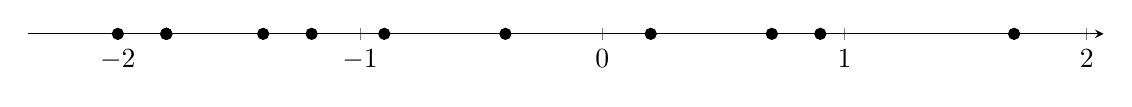
\begin{tikzpicture}[scale=1]
          \begin{axis}[
            axis lines = middle, % boxed, middle
            axis y line=none,
            enlargelimits=true,
            width = {6in},
            % xlabel={\empty}, xlabel style={anchor=west},
            label style={at={(ticklabel* cs:1)}},
            xtick={-2,-1,...,2}, % xticklabels={},
            ]
            \addplot[ only marks, mark=*, mark options={scale=1} ]
              coordinates
              {(1.7,0) (0.7,0) (-0.4,0) (-1.8,0) (0.2,0) (0.9,0) (-1.2,0) (-0.9,0) (-1.8,0) (-1.4,0) (-1.8,0) (-2.0, 0)};
          \end{axis}
        \end{tikzpicture}
      \end{center}
      \blanklines{2}

    \item \textbf{Hypothesis}. ABC causes \underline{\hspace{2in}}.  Some people question our claim and rightly so.

      \begin{quote}
        \faQuestion{} What is the likelihood that \underline{\hspace{3in}}?
        % we are wrong
      \end{quote}

    \item \textbf{Simulation}.  We generate data to replicate the original experiment assuming that ...
      \blanklines{2}

      Therefore, generated data (as a random variable) should 
      \begin{enumerate}
        \item simulate \underline{\hspace{2in}} and, consequently, have an expectation of \underline{\hspace{1cm}}, and
        \item replicate the original experiment and, consequently, have a variance of \underline{\hspace{1cm}}.  
      \end{enumerate}

      \blanklines{3}

      % having mean = 0 means the data comes from the assumption that our hypothesis is false.
      % having the variance matching the original variance is a requirement for replicating the experiment.

    \item \textbf{Conclusion}. We generated \underline{\hspace{1.5cm}} samples and found \underline{\hspace{2cm}} \underline{\hspace{2in}}. Therefore, the probability of committing \underline{\hspace{2in}} is \underline{\hspace{1cm}} which is \underline{\hspace{1in}} the acceptable range of \(5\%\). Therefore, we conclude that our hypothesis should be \underline{\hspace{1in}}.
  \end{itemize}
  \clearpage
  
  How do we actually generate data? How do we calculate \(\mathbb{P}(\text{false positives})\)?

  We assume\footnote{We will not get into why this assumption is valid. It comes from more general statistics theory.}  that the original experiment follows a continuous random variable with PDF \(f(x) = \frac{1}{2a}\) on domain \underline{\hspace{1in}} for some positive constant \(a\).  This PDF determines where the generated data come from.
  \blanklines{5}

  \sout{Let's figure out this constant \(a\).} We already figured out this constant \(a\) in Example~\ref{ex:uniform-distribution-from-mean-and-stddev}.
  \blanklines{5}

  We need to decide what generated replica should be a false positive (because we decided that we want to count false positives in the simulation step).
  \blanklines{10}

  Finally, we can compute \(\mathbb{P}(\text{false positives})\) by repeating the following simulated experiment a large number of times, say \underline{\hspace{2cm}}, and keep track of the total number of false positives we generated.

  Each simulated experiment has two steps.
  \begin{enumerate}
    \item Use pseudorandom variable to generate \(n = 12\) samples following \(U(-a,a)\).
    \item For each replica, decide if we have a false positive.  Keep a count.
  \end{enumerate}
  \blanklines{5}

  We conclude that 
  \[
    \mathbb{P}(\text{false positives}) = \frac{\text{total number of false positives}}{\text{total number of generated replicas}} = 
  \]
\end{example}

\end{document}
